\documentclass[11pt]{article}
\usepackage{amsmath,amssymb,amsthm}
\usepackage{tikz}
\usetikzlibrary{decorations.pathreplacing,calc}
\usepackage[margin=1in]{geometry}
\usepackage{hyperref}

\newcommand{\N}{\mathbb{N}}
\newcommand{\GK}{\operatorname{GK}}
\newcommand{\CPP}{\operatorname{CPP}}
\newcommand{\ALCD}{\operatorname{ALCD}}
\newcommand{\qpoch}[2]{(#1;#2)_\infty}
\newcommand{\qpochn}[3]{(#1;#2)_{#3}}
\newcommand{\qbin}[2]{\genfrac{[}{]}{0pt}{}{#1}{#2}}
\DeclareMathOperator{\wt}{wt}

\theoremstyle{plain}
\newtheorem{theorem}{Theorem}
\newtheorem{conjecture}[theorem]{Conjecture}
\newtheorem{proposition}[theorem]{Proposition}
\newtheorem{lemma}[theorem]{Lemma}
\newtheorem{corollary}[theorem]{Corollary}
\theoremstyle{definition}
\newtheorem{definition}[theorem]{Definition}
\newtheorem{example}[theorem]{Example}
\newtheorem{remark}[theorem]{Remark}
\newtheorem{question}[theorem]{Question}

\title{Proof Strategy: Partial Compression\\
  and the Sign-Reversing Involution}
\author{Robin Langer}
\date{\today}

\begin{document}
\maketitle


%% ============================================================
\section{Setup and notation}
%% ============================================================

Let $c = (c_0, c_1, c_2)$ be a rank-3 profile with
$d = c_0 + c_1 + c_2$ and $3 \nmid d$.
The $Q$-polynomial is
\[
  Q_n = \sum_{S \subseteq \{1,\ldots,n\}}
    (-1)^{|S|}\, q^{\sigma(S)}\, h_{n-|S|},
\]
where $h_m = (q)_m \cdot g_m \in \N[q]$ and
$\sigma(S) = \sum_{s \in S} s$.
Expanding $(q)_m = \sum_{U \subseteq \{1,\ldots,m\}}
(-1)^{|U|} q^{\sigma(U)}$, the full ground set is
\[
  Q_n = \sum_{\substack{S \subseteq \{1,\ldots,n\} \\
    U \subseteq \{1,\ldots,m\} \\ \mu \in \CPP_m(c)}}
    (-1)^{|S|+|U|}\, q^{\sigma(S) + \sigma(U) + |\mu|},
\]
where $m = n - |S|$ and $\CPP_m(c)$ denotes CPPs with
profile~$c$ and $\max(\mu) = m$.


%% ============================================================
\section{Two views of a cylindric plane partition}
\label{sec:two-views}
%% ============================================================

A CPP~$\nu$ with max entry~$n$ and profile $c = (c_0, c_1, c_2)$
lives on a cylindric growth diagram.  The growth diagram encodes
the same data in two equivalent ways: as concentric rings
(the \emph{onion}), or as a tower of horizontal bands
(the \emph{NILP tower}).  We describe both views and the
dictionary between them, using the running example
$c = (2,1,0)$, $\lambda = \bigl((2),(2,1),(1)\bigr)$
with $\max = 2$ and $|\lambda| = 6$.


\subsection{View 1: The onion (concentric rings)}

The growth diagram has $n$~concentric \emph{rings}, numbered
$1$~(innermost) to~$n$~(outermost).  Each ring carries
$d$~face labels---one per face around the cylinder.  The
boundary between consecutive rings is a triple of partitions
(the vertex labels of the growth diagram at that level).

\begin{center}
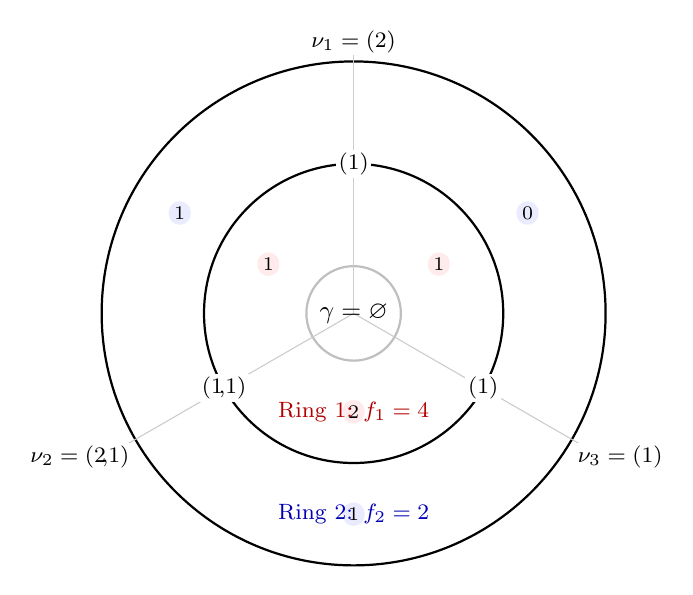
\begin{tikzpicture}[scale=1.0]
  % Concentric circles: levels 0, 1, 2
  \draw[thick, gray!50] (0,0) circle (0.6);
  \draw[thick] (0,0) circle (1.9);
  \draw[thick] (0,0) circle (3.2);

  % Radial lines (3 arcs of the cylinder)
  \foreach \a in {90, 210, 330} {
    \draw[thin, gray!40] (0,0) -- (\a:3.4);
  }

  % Centre label
  \node[font=\small] at (0,0) {$\gamma = \varnothing$};

  % Level 1 partition labels (on middle circle)
  \node[fill=white, inner sep=1pt, font=\footnotesize]
    at (90:1.9) {$(1)$};
  \node[fill=white, inner sep=1pt, font=\footnotesize]
    at (210:1.9) {$(1\!,\!1)$};
  \node[fill=white, inner sep=1pt, font=\footnotesize]
    at (330:1.9) {$(1)$};

  % Level 2 partition labels (on outer circle)
  \node[fill=white, inner sep=1pt, font=\footnotesize,
    above=2pt] at (90:3.2) {$\nu_1 = (2)$};
  \node[fill=white, inner sep=1pt, font=\footnotesize,
    below left=1pt] at (210:3.2) {$\nu_2 = (2\!,\!1)$};
  \node[fill=white, inner sep=1pt, font=\footnotesize,
    below right=1pt] at (330:3.2) {$\nu_3 = (1)$};

  % Face labels: Ring 1 (between circles 0 and 1)
  \node[fill=red!8, rounded corners, inner sep=2pt,
    font=\scriptsize] at (150:1.25) {$1$};
  \node[fill=red!8, rounded corners, inner sep=2pt,
    font=\scriptsize] at (270:1.25) {$2$};
  \node[fill=red!8, rounded corners, inner sep=2pt,
    font=\scriptsize] at (30:1.25) {$1$};

  % Face labels: Ring 2 (between circles 1 and 2)
  \node[fill=blue!8, rounded corners, inner sep=2pt,
    font=\scriptsize] at (150:2.55) {$1$};
  \node[fill=blue!8, rounded corners, inner sep=2pt,
    font=\scriptsize] at (270:2.55) {$1$};
  \node[fill=blue!8, rounded corners, inner sep=2pt,
    font=\scriptsize] at (30:2.55) {$0$};

  % Ring labels
  \node[font=\footnotesize, blue!70!black]
    at (0, -2.55) {Ring 2: $f_2 = 2$};
  \node[font=\footnotesize, red!70!black]
    at (0, -1.25) {Ring 1: $f_1 = 4$};
\end{tikzpicture}
\end{center}

\noindent
Reading from outside in: the outermost boundary carries the
CPP~$\lambda$; the innermost boundary is the base
partition~$\gamma$.  Each ring's face labels encode one
``layer'' of the CPP---how the boundary partitions change from
one level to the next via the Burge local rule.
\textbf{Peeling} ring~$k$ means applying the inverse Burge rule
at all $d$~faces of ring~$k$, extracting the face labels and
collapsing the boundary inward.


\subsection{View 2: The NILP tower (horizontal bands)}

The same data can be ``unrolled'' into a tower of horizontal
bands.  Band~$k$ occupies the strip between levels $k{-}1$
and~$k$.  The $d$~face labels sit inside each band, and the
boundary partition triples label the horizontal lines.

\begin{center}
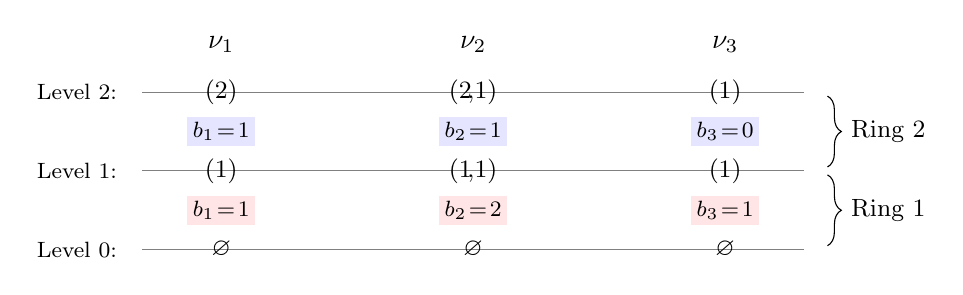
\begin{tikzpicture}[
    level/.style={font=\small},
    face/.style={font=\footnotesize, fill=white, inner sep=2pt},
    >=stealth
  ]
  \def\colsep{3.2}
  \def\rowsep{2.0}

  % Column headers
  \node at (0, 2*\rowsep/2+0.6) {$\nu_1$};
  \node at (\colsep, 2*\rowsep/2+0.6) {$\nu_2$};
  \node at (2*\colsep, 2*\rowsep/2+0.6) {$\nu_3$};

  % Horizontal lines for levels
  \foreach \j in {0,1,2} {
    \draw[gray] (-1.0, \j*\rowsep/2)
      -- (2*\colsep+1.0, \j*\rowsep/2);
  }

  % Level labels on left
  \node[left, font=\footnotesize] at (-1.2, 0)
    {Level 0:};
  \node[left, font=\footnotesize] at (-1.2, \rowsep/2)
    {Level 1:};
  \node[left, font=\footnotesize] at (-1.2, 2*\rowsep/2)
    {Level 2:};

  % Level 0 (bottom) = base
  \node[level] at (0, 0) {$\varnothing$};
  \node[level] at (\colsep, 0) {$\varnothing$};
  \node[level] at (2*\colsep, 0) {$\varnothing$};

  % Level 1 (middle)
  \node[level] at (0, \rowsep/2) {$(1)$};
  \node[level] at (\colsep, \rowsep/2) {$(1\!,\!1)$};
  \node[level] at (2*\colsep, \rowsep/2) {$(1)$};

  % Level 2 (top) = CPP
  \node[level] at (0, 2*\rowsep/2) {$(2)$};
  \node[level] at (\colsep, 2*\rowsep/2) {$(2\!,\!1)$};
  \node[level] at (2*\colsep, 2*\rowsep/2) {$(1)$};

  % Face labels: Ring 1 (between levels 0 and 1)
  \node[face, fill=red!10] at (0, \rowsep/4)
    {$b_1\!=\!1$};
  \node[face, fill=red!10] at (\colsep, \rowsep/4)
    {$b_2\!=\!2$};
  \node[face, fill=red!10] at (2*\colsep, \rowsep/4)
    {$b_3\!=\!1$};

  % Face labels: Ring 2 (between levels 1 and 2)
  \node[face, fill=blue!10] at (0, 3*\rowsep/4)
    {$b_1\!=\!1$};
  \node[face, fill=blue!10] at (\colsep, 3*\rowsep/4)
    {$b_2\!=\!1$};
  \node[face, fill=blue!10] at (2*\colsep, 3*\rowsep/4)
    {$b_3\!=\!0$};

  % Braces for rings
  \draw[decorate, decoration={brace, amplitude=5pt}]
    (2*\colsep+1.3, 2*\rowsep/2-0.05)
    -- (2*\colsep+1.3, \rowsep/2+0.05)
    node[midway, right=5pt, font=\small] {Ring 2};
  \draw[decorate, decoration={brace, amplitude=5pt}]
    (2*\colsep+1.3, \rowsep/2-0.05)
    -- (2*\colsep+1.3, 0.05)
    node[midway, right=5pt, font=\small] {Ring 1};
\end{tikzpicture}
\end{center}

\noindent
The columns correspond to the three partitions
$\nu_1, \nu_2, \nu_3$.  Reading upward from the base, each
band adds one ring's worth of structure.  The partition
boundaries at each level trace \emph{paths} running vertically
through the tower: these are the non-intersecting lattice paths
on the cylinder, and the interlacing conditions ensure they
never cross.


\subsection{The dictionary}

\begin{center}
\renewcommand{\arraystretch}{1.4}
\begin{tabular}{l|l}
\textbf{Concentric rings (onion)}
  & \textbf{NILP tower (bands)}
\\ \hline
Ring $k$ (annular region)
  & Horizontal band at height $k$ \\
Face labels at ring $k$
  & Cell contents in band $k$ \\
Boundary at level $k$
  & Partition triple at height $k$ \\
Outermost boundary (level $n$)
  & Top of tower $=$ CPP $\nu$ \\
Base partition $\gamma$ (level $0$)
  & Bottom of tower \\
Peel ring $k$ (move inward)
  & Remove band, read off face labels \\
Glue ring $k$ (move outward)
  & Add band on top, fill in face labels \\
Inside $\to$ outside
  & Bottom $\to$ top
\end{tabular}
\end{center}

\noindent
The two views are isomorphic representations of the same
growth diagram.  The onion emphasises the nested structure
(removing rings one at a time, like peeling an onion); the
tower emphasises the sequential structure (paths growing
level by level).


\subsection{Compression in both views}

A ground-set element $(S, U, \mu)$ is a \emph{compressed CPP
with max part~$n$}.  The compression has a transparent meaning
in each view.

\begin{center}
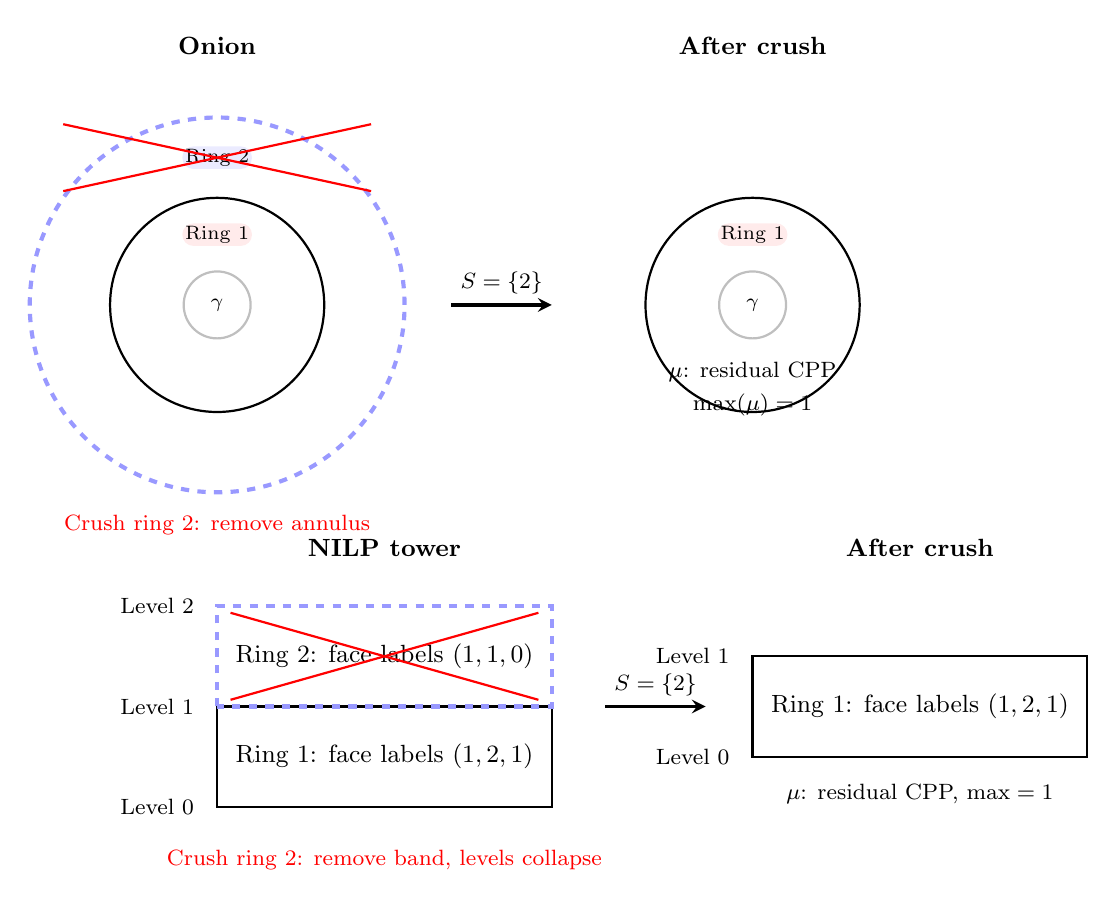
\begin{tikzpicture}[scale=0.85, >=stealth]
  %% === ONION: Before ===
  \node[above, font=\small\bfseries] at (0, 3.6) {Onion};
  \draw[thick, gray!50] (0,0) circle (0.5);
  \draw[thick] (0,0) circle (1.6);
  \draw[thick, blue!40, dashed, line width=1.5pt]
    (0,0) circle (2.8);
  \node[font=\scriptsize] at (0,0) {$\gamma$};
  \node[font=\scriptsize, fill=red!8, rounded corners,
    inner sep=1pt] at (0, 1.05) {Ring 1};
  \node[font=\scriptsize, fill=blue!8, rounded corners,
    inner sep=1pt] at (0, 2.2) {Ring 2};
  % Cross out ring 2
  \draw[red, thick] (-2.3, 1.7) -- (2.3, 2.7);
  \draw[red, thick] (-2.3, 2.7) -- (2.3, 1.7);
  \node[red, font=\footnotesize, below] at (0, -3.0)
    {Crush ring 2: remove annulus};

  %% Arrow
  \draw[->, very thick] (3.5, 0) -- (5.0, 0)
    node[midway, above, font=\footnotesize] {$S = \{2\}$};

  %% === ONION: After ===
  \begin{scope}[xshift=8cm]
    \node[above, font=\small\bfseries] at (0, 3.6)
      {After crush};
    \draw[thick, gray!50] (0,0) circle (0.5);
    \draw[thick] (0,0) circle (1.6);
    \node[font=\scriptsize] at (0,0) {$\gamma$};
    \node[font=\scriptsize, fill=red!8, rounded corners,
      inner sep=1pt] at (0, 1.05) {Ring 1};
    \node[font=\footnotesize] at (0, -1.0)
      {$\mu$: residual CPP};
    \node[font=\footnotesize] at (0, -1.5)
      {$\max(\mu) = 1$};
  \end{scope}

  %% === TOWER: Before ===
  \begin{scope}[yshift=-7.5cm]
    \node[above, font=\small\bfseries] at (2.5, 3.6)
      {NILP tower};
    % Band 1
    \draw[thick] (0, 0) rectangle (5, 1.5);
    \node at (2.5, 0.75)
      {\small Ring 1: face labels $(1,2,1)$};
    % Band 2 (to be crushed)
    \draw[thick, blue!40, dashed, line width=1.5pt]
      (0, 1.5) rectangle (5, 3.0);
    \node at (2.5, 2.25)
      {\small Ring 2: face labels $(1,1,0)$};
    % Cross out band 2
    \draw[red, thick] (0.2, 1.6) -- (4.8, 2.9);
    \draw[red, thick] (0.2, 2.9) -- (4.8, 1.6);
    % Level labels
    \node[left, font=\footnotesize] at (-0.2, 0) {Level 0};
    \node[left, font=\footnotesize] at (-0.2, 1.5) {Level 1};
    \node[left, font=\footnotesize] at (-0.2, 3.0) {Level 2};
    \node[red, font=\footnotesize, below] at (2.5, -0.5)
      {Crush ring 2: remove band, levels collapse};

    %% Arrow
    \draw[->, very thick] (5.8, 1.5) -- (7.3, 1.5)
      node[midway, above, font=\footnotesize] {$S = \{2\}$};

    %% === TOWER: After ===
    \begin{scope}[xshift=8cm]
      \node[above, font=\small\bfseries] at (2.5, 3.6)
        {After crush};
      \draw[thick] (0, 0.75) rectangle (5, 2.25);
      \node at (2.5, 1.5)
        {\small Ring 1: face labels $(1,2,1)$};
      \node[left, font=\footnotesize] at (-0.2, 0.75)
        {Level 0};
      \node[left, font=\footnotesize] at (-0.2, 2.25)
        {Level 1};
      \node[font=\footnotesize] at (2.5, 0.2)
        {$\mu$: residual CPP, $\max = 1$};
    \end{scope}
  \end{scope}
\end{tikzpicture}
\end{center}

\medskip\noindent
\textbf{Crushing} ring~$k$ (adding $k$ to $S$):
\begin{itemize}
  \item In the onion: removes one annulus; adjacent boundaries
    merge.
  \item In the tower: removes one horizontal band; levels above
    collapse downward.
\end{itemize}

\noindent
\textbf{Marking} ring~$i$ (adding $i$ to $U$): thins the
surviving ring without removing it.  In the tower, this
tightens the gap between levels $i{-}1$ and~$i$---the paths
come closer together but do not merge.

\medskip\noindent
The full triple $(S, U, \mu)$ is therefore:
\begin{center}
\renewcommand{\arraystretch}{1.3}
\begin{tabular}{r@{\;:\;}l}
$S \subseteq \{1, \ldots, n\}$
  & which rings are \emph{removed}
    (structural compression) \\
$U \subseteq \{1, \ldots, m\}$
  & which surviving rings are \emph{thinned}
    (weight compression) \\
$\mu \in \CPP_m(c)$
  & the residual CPP on the surviving rings
    ($m = n - |S|$)
\end{tabular}
\end{center}
with sign $(-1)^{|S|+|U|}$ and weight
$\sigma(S) + \sigma(U) + |\mu|$.


%% ============================================================
\section{Why Sch\"utzenberger does not suffice}
%% ============================================================

Let $\sigma$ denote the Sch\"utzenberger involution on CPPs
(evacuation via Burge + inverse RSK).  If $\lambda$
compresses to $(S, U, \mu)$, then $\sigma(\lambda)$
compresses to
\[
  S' = \{n+1-k : k \in S\}, \qquad
  U' = \{m+1-k : k \in U\}, \qquad
  \mu' = \sigma(\mu).
\]
Since $|S'| = |S|$ and $|U'| = |U|$, the sign is preserved:
\[
  (-1)^{|S'|+|U'|} = (-1)^{|S|+|U|}.
\]
\textbf{Conclusion:} $\sigma$ is a sign-preserving involution
on the ground set.  It maps positive elements to positive and
negative to negative.  It cannot serve as the sign-reversing
involution needed to prove $Q_n \in \N[q]$.

\begin{remark}
The fundamental reason is that $\sigma$ is a \emph{global}
operation: it reverses all ring indices simultaneously
($k \mapsto n+1-k$), preserving cardinalities $|S|$ and $|U|$.
A sign-reversing involution must be \emph{local}: it must
change $|S|$ or $|U|$ by exactly~$1$ at each step.
\end{remark}


%% ============================================================
\section{The key idea: partial compression decouples crossings}
%% ============================================================

\subsection*{The problem with geometric swaps}

In the uncompressed state, a ``swap at level~$k$'' means
resolving an actual geometric crossing of lattice paths
on the cylinder.  This is difficult because:
\begin{enumerate}
  \item The paths wrap around (cyclic boundary conditions).
  \item Swapping at level~$k$ can create new crossings at
    other levels.
  \item The face-label interactions between levels are coupled.
\end{enumerate}

\subsection*{The solution: work in the ALCD representation}

The ALCD (ascending level crystal decomposition) of a CPP
$\lambda$ with $\max = n$ records the face labels
$\beta_k = (b_1^{(k)}, b_2^{(k)}, b_3^{(k)})$ at each
ring $k = 1, \ldots, n$.

In the partially compressed state $(S, U, \mu)$
\emph{with the ALCD remembered}, the crossings are
\textbf{decoupled}.  Each ring sits independently in the
ALCD with its face labels, and the ``swap'' reduces to
\textbf{toggling a label}:

\bigskip
\begin{center}
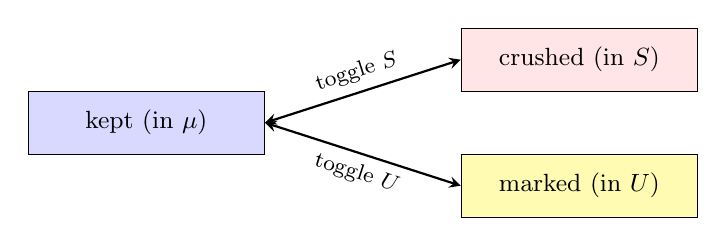
\begin{tikzpicture}[
    box/.style={draw, minimum width=3cm, minimum height=0.8cm,
      font=\small},
    arr/.style={<->, thick, >=stealth}
  ]
  \node[box, fill=blue!15] (kept) at (0, 0) {kept (in $\mu$)};
  \node[box, fill=red!10] (crush) at (5.5, 0.8) {crushed (in $S$)};
  \node[box, fill=yellow!30] (mark) at (5.5, -0.8) {marked (in $U$)};

  \draw[arr] (kept.east) -- (crush.west)
    node[midway, above, font=\footnotesize, sloped]
      {toggle $S$};
  \draw[arr] (kept.east) -- (mark.west)
    node[midway, below, font=\footnotesize, sloped]
      {toggle $U$};
\end{tikzpicture}
\end{center}

\bigskip\noindent
No geometric path resolution is needed.  The face labels
are already recorded in the ALCD---we just change whether
ring~$k$ is counted in $\mu$, absorbed into $\sigma(S)$,
or absorbed into $\sigma(U)$.


%% ============================================================
\section{The arithmetic condition}
%% ============================================================

The sign flip is automatic: each toggle changes $|S|$ or
$|U|$ by~$1$.  The only remaining constraint is
\textbf{weight preservation}.

\begin{definition}[Face-label total]
For ring~$k$ of a CPP~$\lambda$, the \emph{face-label total}
is
\[
  f_k := b_1^{(k)} + b_2^{(k)} + b_3^{(k)},
\]
the total number of parts demoted when peeling ring~$k$.
\end{definition}

The weight effects of each toggle are:

\medskip
\begin{center}
\renewcommand{\arraystretch}{1.3}
\begin{tabular}{l|c|c}
\textbf{Operation} & \textbf{Sign change} &
  \textbf{Weight change} \\ \hline
Crush ring $k$ (add $k$ to $S$) &
  $(-1)$ & $+k - f_k \cdot k'$ \\
Mark ring $k$ (add $k$ to $U$) &
  $(-1)$ & $+k$ \\
\end{tabular}
\end{center}

\medskip\noindent
Here, crushing ring~$k$ adds $k$ to $\sigma(S)$ and
removes ring~$k$'s weight contribution from $|\mu|$.
The net weight change from crushing ring~$k$ is:
\begin{equation}\label{eq:crush-weight}
  \boxed{\;
    \Delta\wt = k - (\text{weight of ring } k \text{ in } \mu).
  \;}
\end{equation}

\textbf{Weight is preserved if and only if the weight of
ring~$k$ in $\mu$ equals $k$.}

\begin{example}[From PEEL-examples]
For $\lambda = \bigl((2),(2,1),(1)\bigr)$ with $c = (2,1,0)$:
\begin{itemize}
  \item Ring~2: face labels $(1,1,0)$, weight of ring~$2$
    is $1 \cdot 2 + 1 \cdot 2 + 0 \cdot 2 = 4$?

    No---the weight of ring~$k$ is the total
    contribution of all cells at height $k$, which is
    $f_k \cdot k$ where $f_k$ is the number of cells.
    So ring~2 contributes $2 \cdot 2 = 4$.  But
    $\Delta\wt = 2 - 4 = -2 \neq 0$.

    Wait---from the PEEL examples, crushing ring~2
    changed weight by $+2 - 2 = 0$ (weight preserved).
    The face-label total is $f_2 = 1 + 1 + 0 = 2$, and
    the weight of ring~$2$ in $\mu$ is the total weight
    of all parts equal to~$2$, which is
    $f_2 \cdot 2 = 4$.  But $\sigma(S)$ gains $+2$,
    and $|\mu|$ loses $4$.  That gives $\Delta = 2 - 4 = -2$.

    Hmm.  But the PEEL example says $\sigma(S) + |\mu|
    = 2 + 4 = 6 = |\lambda|$.  So crushing ring~2
    \emph{does} preserve total weight: the original has
    $|\lambda| = 6$ and the compressed version has
    $\sigma(\{2\}) + |\mu| = 2 + 4 = 6$.

    Resolution: $|\mu|$ is the weight of the residual
    CPP, which is $|\lambda|$ minus the weight of
    ring~$2$.  Weight of ring~$2$ = $f_2 \cdot 2 = 4$?
    No: $|\mu| = |(1)| + |(1,1)| + |(1)| = 1 + 2 + 1
    = 4$.  And $|\lambda| = 2 + 3 + 1 = 6$.
    So ring~$2$ contributes $6 - 4 = 2$ to $|\lambda|$.
    And $\sigma(\{2\}) = 2$.  So $\Delta = 0$. \checkmark

    \textbf{The weight of ring~$k$ is $f_k \cdot 1
    = f_k$} (each cell at height~$k$ contributes~$1$
    to the weight beyond the cells at height~$k-1$).
    No---each part equal to~$k$ contributes $k$ total,
    but the residual $\mu$ retains the parts at
    heights $< k$.

    \textbf{Correct rule:} Crushing ring~$k$ replaces
    each part equal to~$k$ with a part equal to~$k-1$
    (demotion).  This reduces $|\mu|$ by $f_k$ (one
    per demoted part).  And $\sigma(S)$ increases by $k$.
    So
    \[
      \Delta\wt = k - f_k.
    \]
    For ring~2: $\Delta = 2 - 2 = 0$. \checkmark \\
    For ring~1: $\Delta = 1 - 4 = -3$. \checkmark
  \end{itemize}
\end{example}

\begin{proposition}[Crush weight change]
\label{prop:crush}
Crushing ring~$k$ from a CPP~$\mu$ (demoting all $f_k$
parts equal to~$k$) changes the total weight of the
ground-set element by
\[
  \Delta\wt = k - f_k,
\]
where $f_k = b_1^{(k)} + b_2^{(k)} + b_3^{(k)}$ is the
face-label total at ring~$k$.  Weight is preserved if and
only if $f_k = k$.
\end{proposition}

\begin{proof}
Crushing ring~$k$ adds $k$ to $\sigma(S)$.  Each of the
$f_k$ parts equal to~$k$ is demoted to $k-1$, reducing
$|\mu|$ by $f_k$.  Net change: $k - f_k$.
\end{proof}


%% ============================================================
\section{The proof strategy}
%% ============================================================

\begin{definition}[Balanced ring]
Ring~$k$ of a CPP~$\mu$ is \emph{balanced} if $f_k = k$,
i.e., the face-label total at ring~$k$ equals the ring
index.
\end{definition}

The sign-reversing involution $\iota$ on the ground set
would work as follows:

\begin{enumerate}
  \item Given a ground-set element $(S, U, \mu)$ with
    $S \neq \varnothing$ or $U \neq \varnothing$
    (i.e., not a pure CPP with no decorations).
  \item \textbf{Find a balanced ring~$k$} in the ALCD
    of $\mu$ (or in the ALCD of the original CPP, for
    rings in $S$).
  \item \textbf{Toggle ring~$k$}: if $k \in S$, uncrush it
    (remove from $S$, restore in $\mu$); if $k \notin S$,
    crush it (add to $S$, demote in $\mu$).
  \item The sign flips ($|S|$ changes by $\pm 1$) and the
    weight is preserved ($\Delta = k - f_k = 0$).
\end{enumerate}

The fixed points of $\iota$ are elements where no
balanced ring exists to toggle.  These must all have
positive sign for the conjecture to hold.

\begin{conjecture}[Balanced ring existence]
\label{conj:balanced}
For every ground-set element $(S, U, \mu)$ with
$(-1)^{|S|+|U|} = -1$ (negative sign), there exists a
balanced ring that can be toggled to produce a partner
with positive sign at the same total weight.
\end{conjecture}

If true, this would prove Warnaar's Conjecture~2.7
for all rank-3 profiles with $3 \nmid d$.


%% ============================================================
\section{What the ALCD buys us}
%% ============================================================

The ALCD is the correct data structure because it
\textbf{decouples} the crossings:

\bigskip
\begin{center}
\renewcommand{\arraystretch}{1.4}
\begin{tabular}{r|p{5cm}|p{5cm}}
 & \textbf{Uncompressed} & \textbf{Partially compressed}
  \\ \hline
\textbf{Data} &
  Full CPP $\lambda$ (paths on cylinder) &
  ALCD + labels $(S, U)$ \\
\textbf{Swap} &
  Geometric: resolve path crossing &
  Algebraic: toggle a label \\
\textbf{Coupling} &
  Swapping at level $k$ affects other levels &
  Each ring independent \\
\textbf{Weight} &
  Must track path lengths globally &
  Local check: $f_k \stackrel{?}{=} k$ \\
\textbf{Difficulty} &
  Cylindric geometry (hard) &
  Arithmetic condition (tractable)
\end{tabular}
\end{center}

\bigskip\noindent
The geometric problem (resolving crossings on a cylinder)
has been reduced to an arithmetic problem (finding balanced
rings in the ALCD).  The cylindric structure is still
present---it determines the face labels $f_k$---but it no
longer governs the involution mechanism.


%% ============================================================
\section{The marking layer ($U$)}
%% ============================================================

The subset $U \subseteq \{1, \ldots, m\}$ provides
additional flexibility.  Marking ring~$k$ (adding $k$ to $U$)
changes the sign but adds $k$ to the weight unconditionally.
This means:

\begin{itemize}
  \item A \textbf{crush--mark pair} can be weight-preserving
    even when neither operation is individually:
    crush ring~$j$ ($\Delta = j - f_j$) and mark ring~$k$
    ($\Delta = +k$) gives total $\Delta = j - f_j + k$.
    Setting this to zero: $k = f_j - j$.
  \item This extends the reach of the involution: even if
    no single balanced ring exists, a crush--mark pair might
    achieve cancellation.
\end{itemize}

However, a crush--mark pair changes $|S|$ by $+1$ and
$|U|$ by $+1$, so the net sign change is
$(-1)^2 = +1$---\textbf{no sign flip}.
To flip the sign, exactly one of $|S|$ or $|U|$ must
change.  So the involution must use either a single crush
\emph{or} a single mark, not both simultaneously.

\begin{remark}
Marking ring~$k$ is weight-preserving only if $k = 0$,
which is not in $\{1, \ldots, m\}$.  So a pure mark
never preserves weight.  The involution must use
crush/uncrush (toggling $S$), not mark/unmark
(toggling $U$).

The $U$ layer therefore plays a \emph{passive} role:
it changes the effective $m$ (the number of available
rings in $\mu$) and shifts the weight baseline, but
the active pairing mechanism is the crush toggle on $S$.
\end{remark}


%% ============================================================
\section{Open questions}
%% ============================================================

\begin{question}
For which profiles $c$ and which $n$ does every
non-trivially-signed ALCD have a balanced ring?
Equivalently: when is $f_k = k$ achievable for some
ring~$k$?
\end{question}

\begin{question}
Can the involution be defined \emph{canonically}
(e.g., always toggle the smallest balanced ring)?
If so, is it an involution (toggling twice returns to
the original)?
\end{question}

\begin{question}
What is the role of the Sch\"utzenberger involution
$\sigma$ in this framework?  Since $\sigma$ is
sign-preserving, it acts as a symmetry \emph{within}
each sign class.  Does it help identify balanced rings
or constrain the structure of fixed points?
\end{question}

\begin{question}
For $3 \mid d$, the polynomials $h_m$ are no longer in
$\N[q]$ (the ground set is not genuine).  Can the
partial compression framework be adapted using the
modified normalisation
$(q^\ell; q^\ell)_n$ with $\ell = \gcd(d, 3)$?
\end{question}


\end{document}
